%!TEX root = ../template.tex
%%%%%%%%%%%%%%%%%%%%%%%%%%%%%%%%%%%%%%%%%%%%%%%%%%%%%%%%%%%%%%%%%%%%
%% chapter4.tex
%% NOVA thesis document file
%%
%% Chapter with lots of dummy text
%%%%%%%%%%%%%%%%%%%%%%%%%%%%%%%%%%%%%%%%%%%%%%%%%%%%%%%%%%%%%%%%%%%%

\typeout{NT FILE chapter4.tex}%

\chapter{Development Plan}
\label{sec:dev_plan}

The implementation of the proposed \gls{DSL} requires a methodical and objective approach in terms of timing and task management. For that reason, a Gantt chart was made with the intent of guiding the development and ensuring the end product meets expectations. 

\begin{figure}[htbp]
	\centering
	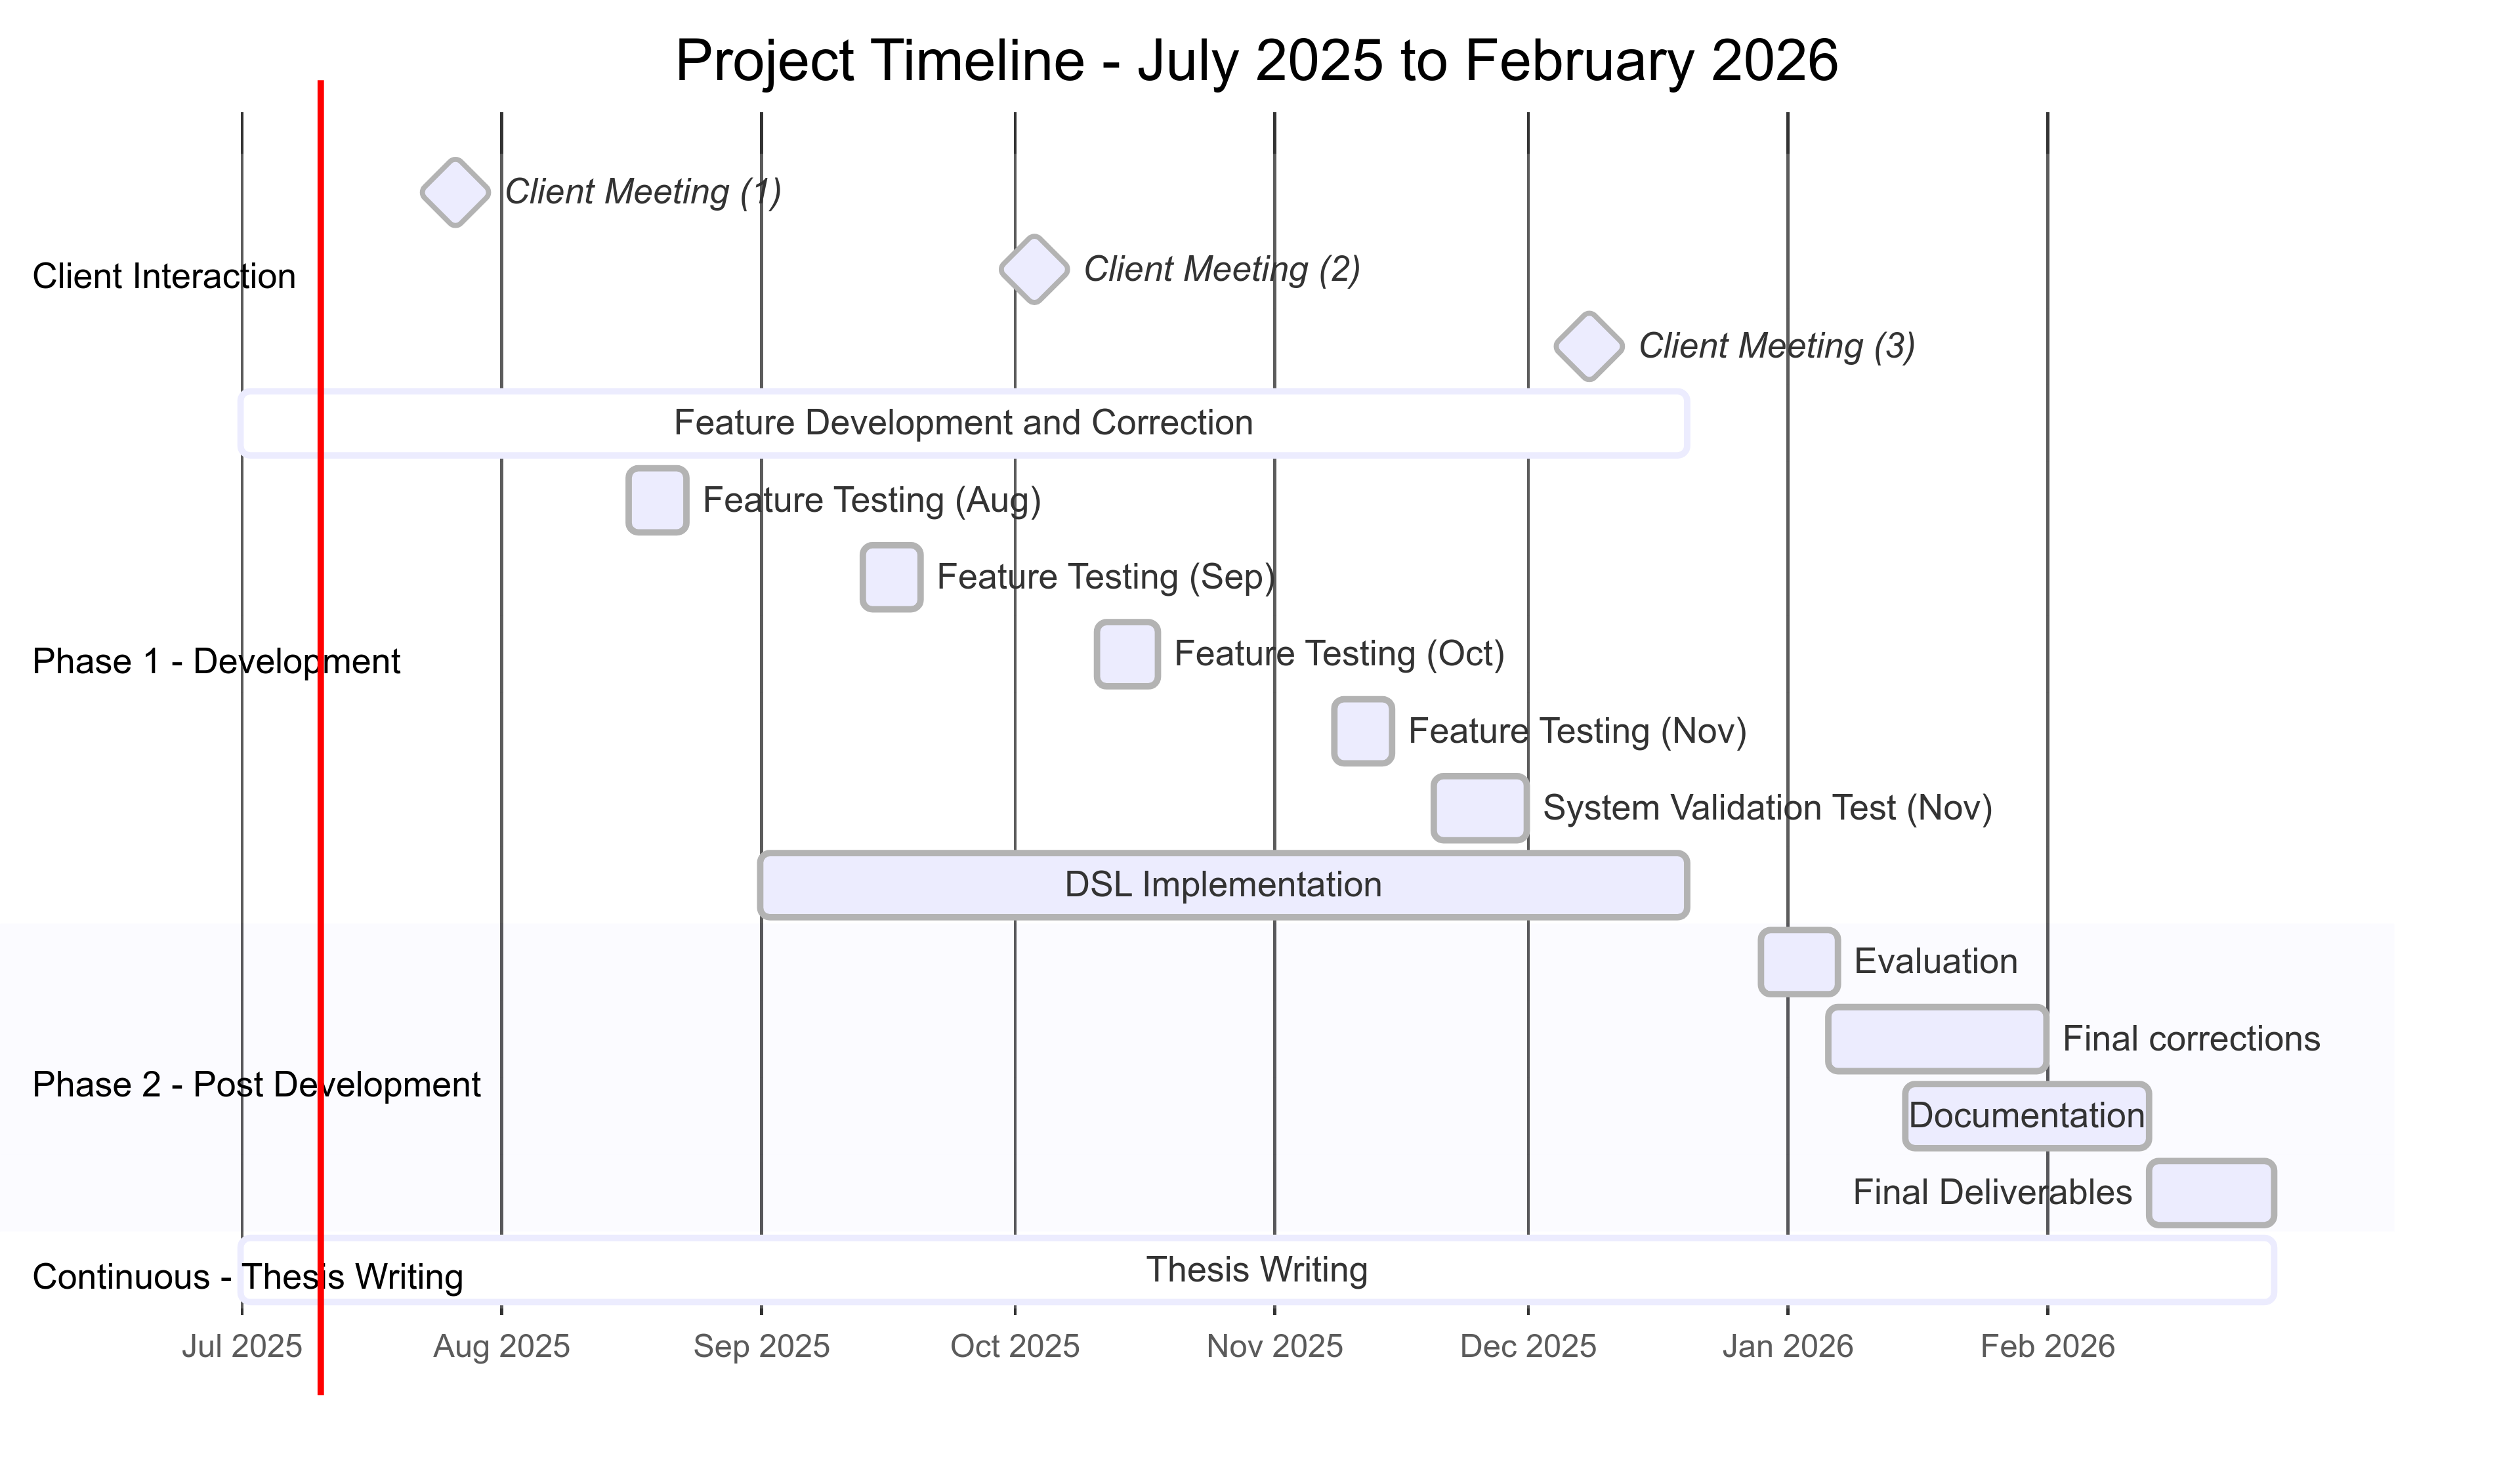
\includegraphics[height=0.63\textwidth]{gantt.png}
	\caption{Thesis planning Gantt chart}
	\label{fig:gantt}
\end{figure}

As we can see in Figure~\ref{fig:gantt}, the plan is separate in two distinct phases: Development and Documentation. Those phases overlap with both client meetings and the writing of the thesis, which is done in parallel with other tasks from start to finish.

\section{Client Interaction}
\label{sec:dev_plan_client}

Client meetings are present to ensure that the features developed are useful and needed addition to the end user. The first and second meeting are mostly interviews directed to acquire quick feedback on the matter, while the third meeting will focus on the evaluation and testing of the mostly finished code generator configurator.

\section{Development Phase}
\label{sec:dev_plan_dev}

The development follows an iterative nature, which means that once a feature is developed, it is tested, documented and corrected when needed. Each month, full system wide testing, is also conducted to ensure multiple features work in harmony with each other. A system integration test is also performed near the end of the development phase to ensure that end users can use the system effectively and can achieve goals unachievable before. This is a critical point in the development since it will be used in addition to the third client meeting to build a system evaluation report.

These will be the types of testing used and their goals:

\begin{itemize}
	\item \textbf{Unit Testing} during development, as new features get developed. Ensures new features meet their goals and catches early bugs.
	\item \textbf{Regression Testing} done monthly to make sure previous features are still working with the addition of new ones.
	\item \textbf{Integration Testing} done in addition to Regression Testing to test how different parts of the system work together.
	\item \textbf{Validation Testing} after development to validate that the features developed are in line with the requests of the end users and clients that will be testing the whole system.
\end{itemize}

Parallel to the code generator configuration feature development, a \gls{DSL} will also be developed. Near the end of the development of a specific feature we need to also implement its actual configuration functionality via the \gls{DSL} which will provide a way for end users to use the configurator, hence its parallel development method which also includes testing. Both the feature and \gls{DSL} development go beyond the last evaluation and testing in order to ensure a safety gap for last minute features or corrections.

\section{Documentation Phase}
\label{sec:dev_plan_doc}

The final phase begins with the analysis of previously gathered evaluation results and insights on end user opinion, thought process and interaction when using the configuration language. Its a very important step since it will allow for quick overview on implementation problems, bugs and other suggestions that might have not been thought of before. After that comes the documentation part for both users and future developers, since the configuration language will be very extensible. Documentation, which includes user manuals, developer guides and system documentation, will also be finished during development, however this interval mainly serves to make sure everything is documented properly.

The final part consists in ensuring every deliverable is correct and ready to send. It mostly include meetings and information exchange with every involved party to validate the work done, while not directed to development or corrections, it provides another safe window to make changes if strictly needed.

\section{Final Considerations}
\label{sec:dev_plan_final}

The overall structure of the Gantt chart is clear and direct, although it provides a detailed and structured timeline, in practice it will serve mostly as a base and the development might end up with unforeseen requirements depending on the necessities of the parts involved, or technical challenges. The chart provides clarity and direction but remains adaptable to eventual changing project needs.
